\documentclass[10pt,a4paper,pdf]{beamer}
\usepackage[utf8x]{inputenc}
\usepackage{ucs}
\usepackage[english]{babel}
\usepackage{amsmath}
\usepackage{algorithmic}
\usepackage{tikz}
\usetikzlibrary{shapes,arrows}
\usetikzlibrary{positioning, shapes}
\usetikzlibrary{trees,calc}
\usepackage{fancybox}
\usepackage{tikz-qtree}

\usepackage{amsfonts}
\usepackage{amssymb}
\author{Guillaume Maudoux \& Cédric Libert}
\title{Symbolic search}
\setbeamertemplate{navigation symbols}{}

\renewcommand{\t}[1]{\text{#1}}

%%%%%%%%%%%%%%%%%%%%%%%%%%%%%%%%%%%%%%%%%%%%%%%%%%%%%%%%%%%%%%%%%
%% The following definitions are to extend the LaTeX algorithmic 
%% package with SWITCH statements and one-line structures.
%% The extension is by 
%%   Prof. Farn Wang 
%%   Dept. of Electrical Engineering, 
%%   National Taiwan University. 
%% 
\newcommand{\CASEOF}[1]{\STATE \textbf{case} (#1)}
\newcommand{\ENDCASEOF}{\STATE \textbf{end case}}
\newcommand{\CASE}[1]{\STATE \textbf{of} #1\textbf{:} \begin{ALC@g}}
\newcommand{\ENDCASE}{\end{ALC@g}}
%% 
%% End of the LaTeX algorithmic package extension.
%%%%%%%%%%%%%%%%%%%%%%%%%%%%%%%%%%%%%%%%%%%%%%%%%%%%%%%%%%%%%%%%%

\begin{document}
\tikzstyle{line} = [draw, -latex']
\tikzstyle{feuille} = [rectangle]
\tikzstyle{decision} = [rectangle, draw, fill=gray!20, align=center,
     text centered, minimum height=1cm,minimum width=1cm, node distance=1cm]	
\maketitle
%\begin{frame}
%\tableofcontents
%\end{frame}
%\section{Intro}
%\begin{frame}
%\frametitle{The problem of storing many states}
%
%The list of states still to explore in a classical search can be very space-consuming (exponential in BFS).  One solution is to use DFS, but then memory usage is suboptimal.  We explore another structure able to store many states in a compressed way: the binary decision diagrams.
%
%\end{frame}

\begin{frame}[t]
\frametitle{Binary decision diagrams encode boolean functions}

Boolean function: $F:\{0,1\}^n \rightarrow \{0,1\}$\\[0.5cm]
(RO)BDDs seen as reduced decision trees\\[0.5cm]
 \begin{center}
$f( x = \langle a,b,c \rangle) \ =\  a \lor b \lor c$
 \end{center}
 \pause

  \begin{overlayarea}{6cm}{1cm}
  	\only<2-3>{\begin{tikzpicture}
[every tree node/.style={draw,circle},
   level distance=1.25cm,sibling distance=.5cm, 
   edge from parent path={(\tikzparentnode) -- (\tikzchildnode)}]
\Tree [.\node(a) {a}; 
     \edge node[auto=right] {1};[.\node (b) {b};
        \edge node[auto=right] {1};[.c 
           \edge node[auto=right] {1}; [.\node[feuille] (t1) {1}; ] \edge node[auto=left] {0}; [.\node[feuille] (t2) {1}; ] 
        ]      
        \edge node[auto=left] {0};[.c 
          \edge node[auto=right] {1}; [.\node[feuille] (t3) {1}; ] \edge node[auto=left] {0}; [.\node[feuille] (t4) {1}; ] 
        ] 
    ]
      \edge node[auto=left] {0}; [.b
        \edge node[auto=right] {1}; [.c 
          \edge node[auto=right] {1}; [.\node[feuille] {1}; ] \edge node[auto=left] {0}; [.\node[feuille] {1}; ] 
        ] 
        \edge node[auto=left] {0}; [.c 
          \edge node[auto=right] {1}; [.\node[feuille] {1}; ] \edge node[auto=left] {0}; [.\node[feuille]{0}; ] 
        ]
    ] ]
        \onslide<3>{\draw[red,thick,dotted] ($(t1.north west)+(-0.3,0.3)$)  rectangle ($(t4.south east)+(0.3,-0.3)$);}
\end{tikzpicture}}
\only<4-5>{\begin{tikzpicture}
[every tree node/.style={draw,circle},
   level distance=1.25cm,sibling distance=.5cm, 
   edge from parent path={(\tikzparentnode) -- (\tikzchildnode)}]
\Tree [.\node (a) {a}; 
     \edge[white] node[auto=right] {1};[.\node[white] (b) {1};
        \edge[white];[.\node[white] (c) {c}; 
           \edge[white] node[auto=right] {1}; [.\node[feuille,white] (t1) {1}; ] \edge[white] node[auto=left] {0}; [.\node[feuille] (t2) {1}; ] 
        ]      
        \edge[white] node[auto=left] {0};[.\node[white] (c2) {c}; 
          \edge[white] node[auto=right] {1}; [.\node[feuille,white] (t3) {1}; ] \edge[white] node[auto=left] {0}; [.\node[feuille,white] (t4) {1}; ] 
        ] 
    ]
      \edge node[auto=left] {0}; [.b
        \edge node[auto=right] {1}; [.c 
          \edge node[auto=right] {1}; [.\node[feuille] (t5) {1}; ] \edge node[auto=left] {0}; [.\node[feuille] (t6) {1}; ] 
        ] 
        \edge node[auto=left] {0}; [.c 
          \edge node[auto=right] {1}; [.\node[feuille] {1}; ] \edge node[auto=left]  {0}; [.\node[feuille]{0}; ] 
        ]
    ] ]
        		\draw (a) -- node[above] {1} (t2);

        \onslide<2>{\draw[red,thick,dotted] ($(t1.north west)+(-0.3,0.6)$)  rectangle ($(t4.south east)+(0.3,-0.6)$);}
        \onslide<5>{\draw[red,thick,dotted] ($(t5.north west)+(-0.3,0.3)$)  rectangle ($(t6.south east)+(0.3,-0.3)$);}
\end{tikzpicture}}
\only<6-7>{\begin{tikzpicture}
[every tree node/.style={draw,circle},
   level distance=1.25cm,sibling distance=.5cm, 
   edge from parent path={(\tikzparentnode) -- (\tikzchildnode)}]
\Tree [.\node (a) {a}; 
     \edge[white] node[auto=right] {1};[.\node[white] (b) {1};
        \edge[white];[.\node[white] (c) {c}; 
           \edge[white] node[auto=right] {1}; [.\node[feuille,white] (t1) {1}; ] \edge[white] node[auto=left] {0}; [.\node[feuille] (t2) {1}; ] 
        ]      
        \edge[white] node[auto=left] {0};[.\node[white] (c2) {c}; 
          \edge[white] node[auto=right] {1}; [.\node[feuille,white] (t3) {1}; ] \edge[white] node[auto=left] {0}; [.\node[feuille,white] (t4) {1}; ] 
        ] 
    ]
      \edge node[auto=left] {0}; [.\node (b2) {b};
        \edge node[auto=right] {1}; [.\node[feuille] (c4) {1};
          \edge[white] node[auto=right] {1}; [.\node[feuille,white] (t5) {1};] \edge[white] node[auto=left] {0}; [.\node[feuille,white] (t6) {1}; ] 
        ] 
        \edge node[auto=left] {0}; [.\node (c5) {c}; 
          \edge node[auto=right] {1}; [.\node[feuille] (t7) {1}; ] \edge node[auto=left]  {0}; [.\node[feuille] (t8) {0}; ] 
        ]
    ] ]
        \draw (a) -- node[above] {1} (t2);
        \onslide<2>{\draw[red,thick,dotted] ($(t1.north west)+(-0.3,0.6)$)  rectangle ($(t4.south east)+(0.3,-0.6)$);}
        \onslide<4>{\draw[red,thick,dotted] ($(t7.north west)+(-0.3,0.6)$)  rectangle ($(t8.south east)+(0.3,-0.6)$);}
        
        \onslide<7>{
        	\foreach \name in {t2,c4,t7}
        	  \draw[red,thick,dotted] ($(\name.north west)+(-0.3,0.3)$)  rectangle ($(\name.south east)+(0.3,-0.3)$);}        
\end{tikzpicture}}
\only<8->{\begin{tikzpicture}
[every tree node/.style={draw,circle},
   level distance=1.25cm,sibling distance=.5cm, 
   edge from parent path={(\tikzparentnode) -- (\tikzchildnode)}]
\Tree [.\node (a) {a}; 
     \edge[white] node[auto=right] {1};[.\node[white] (b) {1};
        \edge[white];[.\node[white] (c) {c}; 
           \edge[white] node[auto=right] {1}; [.\node[feuille,white] (t1) {1}; ] \edge[white] node[auto=left] {0}; [.\node[feuille,white] (t2) {1}; ] 
        ]      
        \edge[white] node[auto=left] {0};[.\node[white] (c2) {c}; 
          \edge[white] node[auto=right] {1}; [.\node[feuille,white] (t3) {1}; ] \edge[white] node[auto=left] {0}; [.\node[feuille,white] (t4) {1}; ] 
        ] 
    ]
      \edge node[auto=left] {0}; [.\node (b2) {b};
        \edge[white] node[auto=right] {1}; [.\node[white] (c4) {1};
          \edge[white] node[auto=right] {1}; [.\node[feuille,white] (t5) {1};] \edge[white] node[auto=left] {0}; [.\node[feuille,white] (t6) {1}; ] 
        ] 
        \edge node[auto=left] {0}; [.\node (c5) {c}; 
          \edge node[auto=right] {1}; [.\node[feuille] (t7) {1}; ] \edge node[auto=left]  {0}; [.\node[feuille] (t8) {0}; ] 
        ]
    ] ]
    		\foreach \name in {a,b2}
    			\draw (\name) -- node[above] {1} (t7);
        \onslide<2>{\draw[red,thick,dotted] ($(t1.north west)+(-0.3,0.6)$)  rectangle ($(t4.south east)+(0.3,-0.6)$);}
        \onslide<4>{\draw[red,thick,dotted] ($(t7.north west)+(-0.3,0.6)$)  rectangle ($(t8.south east)+(0.3,-0.6)$);}
        
        \onslide<6>{
        	\foreach \name in {b,c4,t7}
        	  \draw[red,thick,dotted] ($(\name.north west)+(-0.3,0.3)$)  rectangle ($(\name.south east)+(0.3,-0.3)$);} 
    
\end{tikzpicture}}


  \end{overlayarea}


\end{frame}
\section{Representing  state sets with BDDs}
\begin{frame}[t]
\frametitle{From a state set to a BDD}
	% BDDs use boolean vectors $\rightarrow$  states should be boolean vectors\\[0.5cm]\pause
\begin{minipage}[t]{.42\linewidth}
State x = $\langle x_1,x_2 \rangle$,\\
 with $x_1,x_2\in \{0,1\}$\\[0.3cm]	
	\begin{tikzpicture}
	\node[decision](d1) {};
	\foreach \rightof/\name in {d1/d2,d2/d3,d3/d4}{
		\node[decision,right of=\rightof] (\name) {};}
	\node[above of=d1] {init};
	\node[above of=d4] {goal};
	\foreach \couche/\pos/\name/\state in {2/d1/s1/00,3/d2/s2/01,4/d3/s3/10,5/d4/s4/11}{		
		\only<\couche>{\draw[red,fill=red] ($(\pos.north west)+(0.5,-0.5)$)  circle (0.1cm);
		\node[below of=\pos] (\name) {\state};}}
		
	\foreach \couche/\pos/\name/\state in {2/d1/s1/00,3/d2/s2/01,4/d3/s3/10,5/d4/s4/11}{		
		\only<6->{\node[below of=\pos] (\name) {\state};}}
		
			\only<8-10>{\draw[red,fill=red] ($(d2.north west)+(0.5,-0.5)$)  circle (0.1cm);}

	\end{tikzpicture}
\only<7->{
  \vspace*{1cm}
  \begin{itemize}
		%\item allowed states: S(x)
		%\item successor set: Succ(x)
		%\item initial state: $\phi_{\{s\}}(x)$
		%\item goal set: $\phi_T(x)$
		%\item a search frontier: Open(x)
		%\item the transition relation: Trans(x,x')
    \item initial state: $\phi_{\{s\}}(x)$
  \only<8->{
    \item a search frontier: Open(x)
  }
  \only<12->{
    \item the transition relation: Trans(x,x')
  }
  \end{itemize}
}

\end{minipage}%
\only<12->{%
 \begin{minipage}[t]{.54\linewidth}
 \begin{center}
Transition relation
%Set of initial states\\[0.3cm]
%
\begin{tikzpicture}
[every tree node/.style={draw,circle},
   level distance=1.25cm,sibling distance=.5cm, 
   edge from parent path={(\tikzparentnode) -- (\tikzchildnode)}]
\Tree [.\node (x) {$x_1$};
         \edge node[auto=right] {1};
           [.\node (y) {$x_2$};
             \edge node[auto=right] {0};
               [.\node (y'1) {$x_2'$};
                  \edge node[auto=right] {1};
                  	\node[feuille] {1};
                  \edge node[auto=left] {0};
                  	\node[feuille] {0};               
               ]
             \edge node[auto=left] {1};
               [.\node (x') {$x_1'$};
                \edge node[auto=right] {0}; 
                  \node[feuille] {0};
                \edge node[auto=left] {1};
                 [.\node (y') {$x_2$'};
                   \edge node[auto=right] {0};
                   	\node[feuille] {1};
                   \edge node[auto=left] {1};
                   	\node[feuille] {0};
                 ]
               ]
           ]
         \edge node[auto=left] {0};
           [.\node (y2) {$x_2$};
             \edge node[auto=left] {0};
               [.\node (x'2) {$x_1$'};
               	\edge node[auto=right] {1}; 
                  \node[feuille] {0};
                \edge node[auto=left] {0};
                 [.\node (y'2) {$x_2$'};
                   \edge node[auto=right] {0};
                   	\node[feuille] {0};
                   \edge node[auto=left] {1};
                   	\node[feuille] {1};
                 ]
               ]
           ]
	  ]
	\draw (y2) -- node[left] {1} (y');
	\only<10-> {
		\foreach \name in {x,y2,y'}
			\draw[red,thick] (\name) circle (0.5cm);
			 
	}
	
\end{tikzpicture}

 \end{center}
\end{minipage}}%\\[-2cm]
\only<7>{ \begin{minipage}[t]{.54\linewidth}

\begin{center}
Initial state set

\begin{tikzpicture}
[every tree node/.style={draw,circle},
   level distance=1.25cm,sibling distance=.5cm, 
   edge from parent path={(\tikzparentnode) -- (\tikzchildnode)}]
\Tree [.\node (x) {$x_1$};
	            \edge[white] node[auto=left] {1}; [.\node[white] {};]      
        \edge node[auto=left] {0};
        [.\node (y) {$x_2$}; 
          \edge node[auto=right] {1}; [.\node[feuille] (t3) {0}; ] 
          \edge node[auto=left] {0}; [.\node[feuille] (t4) {1}; ]    
     ]]
     
    \draw (x) -- node[left] {1} (t3);
\end{tikzpicture}
\end{center}
\end{minipage}}
\only<8-11>{\begin{minipage}[t]{.54\linewidth}
\begin{center}
Search frontier of state (0,1)

\only<8-9>{\begin{tikzpicture}
[every tree node/.style={draw,circle},
   level distance=1.25cm,sibling distance=.5cm, 
   edge from parent path={(\tikzparentnode) -- (\tikzchildnode)}]
\Tree [.\node (x) {$x_1$};
	            \edge node[auto=right] {1}; 
	            [.\node (y1) {$x_2$};
					\edge node[auto=right] {1}; \node[feuille] {0};
					\edge node[auto=left] {0};  \node[feuille] {1};          
	            ]      
        	        \edge node[auto=left] {0};
                [.\node (y2) {$x_2$};
					\edge node[auto=right] {1}; \node[feuille] {0};
					\edge node[auto=left] (t4) {0};  \node[feuille] {1};          
	            ]
    ]
     \only<9>{\draw[red,thick,dotted] ($(y1.north west)+(-0.5,0.3)$)  rectangle ($(t4.south east)+(0,-1)$);}
\end{tikzpicture}}



\only<10>{\begin{tikzpicture}
[every tree node/.style={draw,circle},
   level distance=1.25cm,sibling distance=.5cm, 
   edge from parent path={(\tikzparentnode) -- (\tikzchildnode)}]
\Tree   [ .\node(x1) {$x_1$}; 
			[.\node (y1) {$x_2$};
					\edge node[auto=right] {1}; \node[feuille] {0};
   					\edge node[auto=left] {0};  \node[feuille] {1};          
        		] 
        	]      
\end{tikzpicture}}

\only<11>{\begin{tikzpicture}
[every tree node/.style={draw,circle},
   level distance=1.25cm,sibling distance=.5cm, 
   edge from parent path={(\tikzparentnode) -- (\tikzchildnode)}]
\Tree   [.\node (y1) {$x_2$};
					\edge node[auto=right] {1}; \node[feuille] {0};
   					\edge node[auto=left] {0};  \node[feuille] {1};          
        ]      
 
\end{tikzpicture}}
\end{center}
\end{minipage}}
%	\begin{itemize}	
%	\item How do we represent a state ? A set of states ? A transition function ?
%	\item Discussion about space efficiency.
%	\end{itemize}
\end{frame}

\section{Computing with BDDs}

\begin{frame}
\frametitle{Variable ordering}

The size $|G|$ of a BDD is the number of nodes in $G$.\\
It is heavily dependent on the order of the variables.

For $f(x_1, \ldots, x_8) = (x_1 \land x_2) \lor \ldots \lor (x_7 \land x_8)$, we can have...

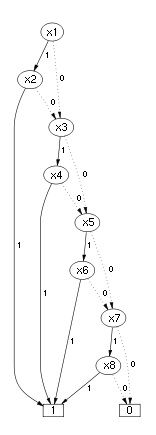
\includegraphics[height=6cm]{images/good.png}
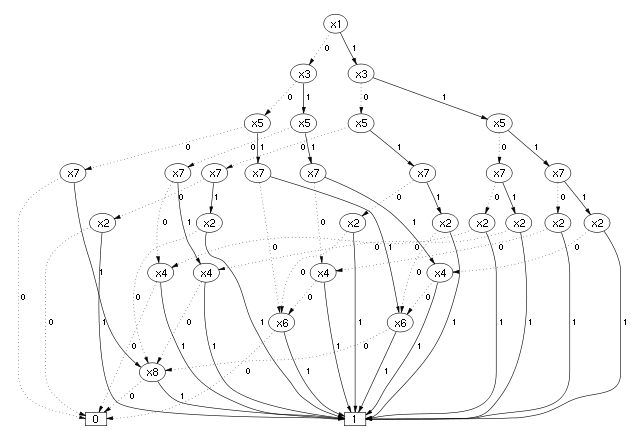
\includegraphics[height=6cm]{images/bad.png}

{\tiny\copyright Dirk Beyer -- wikimedia}

\end{frame}

\begin{frame}
\frametitle{Considerations about the size of BDD's}

The state space is exponential in $n$.

$x = \langle x_1, \ldots, x_n \rangle \in \{0,1\}^n$

$|\{0,1\}^n| = 2^n$

\begin{itemize}
\item Some BDD have no good ordering (all are exponential).
\item We expect $|G|$ to be in $\t{POLY}(n)$, with $n$ the number of variables.\\
This can be proven in some cases.
\pause
\item But finding the optimal variable ordering is NP-Complete
\end{itemize}
\pause
\begin{center}
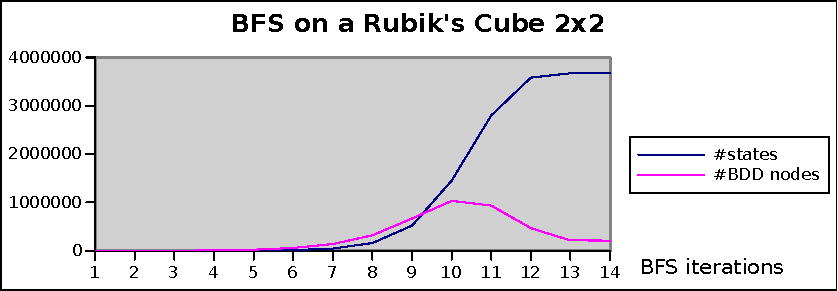
\includegraphics[height=3cm]{images/exponential.pdf}
\end{center}

\begin{center}

\end{center}

\end{frame}

\begin{frame}
\frametitle{Negation of a BDD: inverting the leaves in O(1)}
\begin{center}

\only<1-2>{
\begin{tikzpicture}
[every tree node/.style={draw,circle},
   level distance=1.25cm,sibling distance=.5cm, 
   edge from parent path={(\tikzparentnode) -- (\tikzchildnode)}]
\Tree [.\node (x) {$x_1$};
	            \edge[white] node[auto=left] {1}; [.\node[white] {};]      
        \edge node[auto=left] {0};
        [.\node (y) {$x_2$}; 
          \edge node[auto=right] {1}; [. \node[feuille] (t3) {\only<1>{0}\only<2>{1}}; ] 
          \edge node[auto=left] {0}; [.\node[feuille] (t4) {\only<1>{1}\only<2>{0}}; ]    
     ]]
     
    \draw (x) -- node[left] {1} (t3);
\end{tikzpicture}
}

\end{center}

\end{frame}



\begin{frame}
\frametitle{Intersection of BDDs in $O(|G_f||G_g|)$}
\begin{minipage}[t]{.36\linewidth}
\begin{tikzpicture}
[every tree node/.style={draw,circle},
   level distance=1.25cm,sibling distance=.5cm, 
   edge from parent path={(\tikzparentnode) -- (\tikzchildnode)}]
\Tree [.\node (x) {x};
	            \edge node[auto=right] {1}; 
	            	[.\node (z) {z};
					\edge node[auto=right] {1};
					\node[feuille] (f1) {0};
					\edge node[auto=right] {0};
					\node[feuille] (f2) {1};	 	            	
	            	]      
        ]
     
    \draw (x) edge[bend left] node[right] {0} (f2);
\end{tikzpicture}
\begin{tikzpicture}
[every tree node/.style={draw,circle},
   level distance=1.25cm,sibling distance=.5cm, 
   edge from parent path={(\tikzparentnode) -- (\tikzchildnode)}]
\Tree [.\node (x) {x};
	            \edge node[auto=right] {1}; 
	            	[.\node (y) {y};
					\edge node[auto=right] {1};
					\node[feuille] (f1) {1};
					\edge node[auto=right] {0};
					\node[feuille] (f2) {0};	 	            	
	            	]      
        ]
     
    \draw (x) edge[bend left] node[right] {0} (f2);
\end{tikzpicture}\\[0.1cm]
\only<3-4>{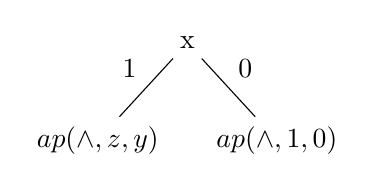
\begin{tikzpicture}
[
   level distance=1.25cm,sibling distance=.5cm, 
   edge from parent path={(\tikzparentnode) -- (\tikzchildnode)}]
\Tree [.\node (x) {x};
	            \edge node[auto=right] {1}; \node (y) {$ap(\wedge,z,y)$};
	            	\edge node[auto=left] {0}; \node {$ap(\wedge,1,0)$};      
        ]
     
\end{tikzpicture}}
\only<5-6>{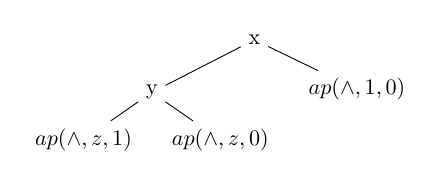
\begin{tikzpicture}
[scale=0.8,
   level distance=0.8cm,sibling distance=.4cm, 
   edge from parent path={(\tikzparentnode) -- (\tikzchildnode)}]
\Tree [.\node (x) {x};
	            [.y $ap(\wedge,z,1)$ $ap(\wedge,z,0)$ ]
	    \node {$ap(\wedge,1,0)$};      
       ]
     
\end{tikzpicture}}
\only<7-8>{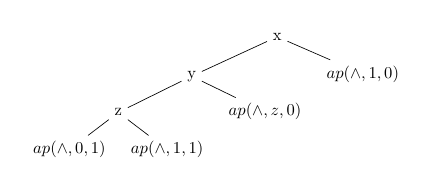
\begin{tikzpicture}
[scale=0.6,
   level distance=0.8cm,sibling distance=.3cm, 
   edge from parent path={(\tikzparentnode) -- (\tikzchildnode)}]
\Tree [.\node (x) {x};
	            [.y [.z $ap(\wedge,0,1)$ $ap(\wedge,1,1)$ ] $ap(\wedge,z,0)$ ]
	    \node {$ap(\wedge,1,0)$};      
       ]
     
\end{tikzpicture}}
\only<9-10>{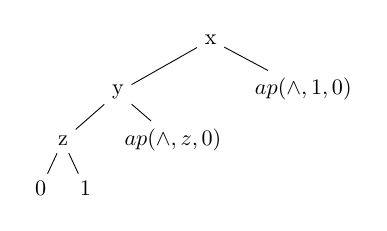
\begin{tikzpicture}
[scale=0.8,
   level distance=0.8cm,sibling distance=.3cm, 
   edge from parent path={(\tikzparentnode) -- (\tikzchildnode)}]
\Tree [.\node (x) {x};
	            [.y [.z 0 1 ] $ap(\wedge,z,0)$ ]
	    \node {$ap(\wedge,1,0)$};      
       ]
     
\end{tikzpicture}}
\only<11->{\begin{tikzpicture}
[
   level distance=0.8cm,sibling distance=.3cm, 
   edge from parent path={(\tikzparentnode) -- (\tikzchildnode)}]
\Tree [.\node (x) {x};
	            [.y [.z 0 1 ] 0 ]
	    			0      
       ]
     
\end{tikzpicture}}

\end{minipage}\hfill
\begin{minipage}[c]{.55\linewidth}
\begin{small}
apply($\wedge,bdd1,bdd2$)
	\begin{algorithmic}
\CASEOF{bdd1,bdd2}
	\pause
	\CASE{(\begin{tikzpicture}[scale=0.7,level distance=0.6cm,sibling distance=.2cm, edge from parent path={(\tikzparentnode) -- (\tikzchildnode)}]\Tree [.$c$ $e_1$ $e_1'$ ]\end{tikzpicture},\begin{tikzpicture}[scale=0.7,level distance=0.6cm,sibling distance=.2cm, edge from parent path={(\tikzparentnode) -- (\tikzchildnode)}]\Tree [.$c$ $e_2$ $e_2'$ ]\end{tikzpicture})}
	\STATE reduce(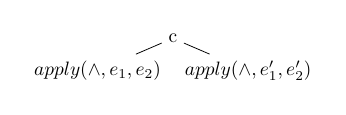
\begin{tikzpicture}[scale=0.7,level distance=0.6cm,sibling distance=.2cm, edge from parent path={(\tikzparentnode) -- (\tikzchildnode)}]\Tree [.c $apply(\wedge,e_1,e_2)$ $apply(\wedge,e_1',e_2')$ ])\end{tikzpicture})
	\ENDCASE
	\pause\pause
	\CASE{(bdd1,\begin{tikzpicture}[scale=0.7,level distance=0.6cm,sibling distance=.2cm, edge from parent path={(\tikzparentnode) -- (\tikzchildnode)}]\Tree [.c $e_2$ $e_2'$ ]\end{tikzpicture}) where $bdd1 < c$}
		\STATE reduce(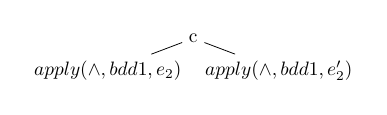
\begin{tikzpicture}[scale=0.7,level distance=0.6cm,sibling distance=.2cm, edge from parent path={(\tikzparentnode) -- (\tikzchildnode)}]\Tree [.c $apply(\wedge,bdd1,e_2)$ $apply(\wedge,bdd1,e_2')$ ]\end{tikzpicture})
	\ENDCASE
	\pause\pause
	\CASE{(\begin{tikzpicture}[scale=0.7,level distance=0.6cm,sibling distance=.2cm, edge from parent path={(\tikzparentnode) -- (\tikzchildnode)}]\Tree [.c $e_1$ $e_1'$ ]\end{tikzpicture},bdd2) where $bdd2 < c$}
		\STATE reduce(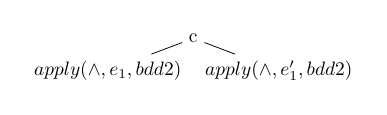
\begin{tikzpicture}[scale=0.7,level distance=0.6cm,sibling distance=.2cm, edge from parent path={(\tikzparentnode) -- (\tikzchildnode)}]\Tree [.c $apply(\wedge,e_1,bdd2)$ $apply(\wedge,e_1',bdd2)$ ]\end{tikzpicture})
	\ENDCASE
	\pause\pause
	\CASE{(0$|$1,0$|$1)}
		\STATE reduce(bdd1 $\wedge$ bdd2)
	\ENDCASE
	\pause\pause
\ENDCASEOF
	\end{algorithmic}
%	\begin{tikzpicture}
\end{small}

%	\end{tikzpicture}
\end{minipage}

%Complexity: $O(|bdd1||bdd2|)$
%\begin{itemize}
%\item union, intersection: $O(|G_f||G_g|)$
%\item projection:
%\item quantification:
%\item time complexity of these operations
%\end{itemize}

\end{frame}

\begin{frame}[c]
\frametitle{Quantification over a BDD in $O(|G_f|^2)$}

Existential quantification($BDD_f$,$x_i$): $BDD_{f[x_i=0]}\vee BDD_{f[x_i=1]}$

\pause
\begin{minipage}[l]{.35\linewidth}
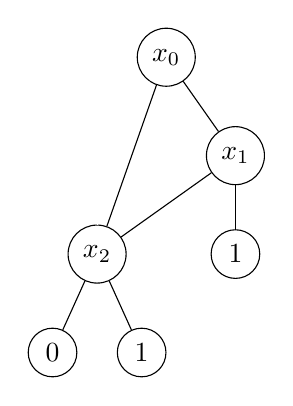
\begin{tikzpicture}
[every tree node/.style={draw,circle},
   level distance=1.25cm,sibling distance=.5cm, 
   edge from parent path={(\tikzparentnode) -- (\tikzchildnode)}]
\Tree [.\node (x) {$x_0$}; \edge[white];
		[.\node[white](y1) {}; \edge[white]; [.\node(z) {$x_2$}; 0 1 ] ]
		[.\node(y) {$x_1$}; 1 ]	  
	  ]
     
    \draw (y) -- (z);
    \draw (x) -- (z);
\end{tikzpicture}
\end{minipage}\pause
\begin{minipage}[c]{.1\linewidth}
$\exists x_0 :$
\end{minipage}\pause
\begin{minipage}[r]{.35\linewidth}
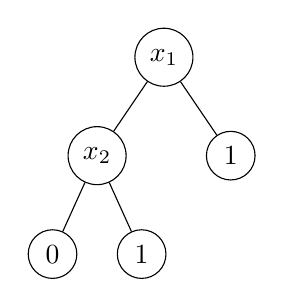
\begin{tikzpicture}
[every tree node/.style={draw,circle},
   level distance=1.25cm,sibling distance=.5cm, 
   edge from parent path={(\tikzparentnode) -- (\tikzchildnode)}]
\Tree 
		[.\node(y) {$x_1$};  [.\node(z) {$x_2$}; 0 1 ]  1 ]
     
\end{tikzpicture}
\end{minipage}\pause
\vspace{0.5cm}

Universal quantification($BDD_f$,$x_i$): $BDD_{f[x_i=0]}\wedge BDD_{f[x_i=1]}$

\end{frame}

\begin{frame}
\frametitle{Computing the successors of a state set in $O((|G_f||G_g|)^2)$}
Given:
\begin{itemize}
\item a state set $\phi_S(x)$
\item a transition relation $Trans(x,x')$
\end{itemize}
\vspace*{2\baselineskip}

Then:
\[ Succ_S(x) = \exists x(\phi_S(x) \land Trans(x,x')) [ x \leftrightarrow x' ] \]

\end{frame}

\section{The BFS implemented with set operations}
\begin{frame}
\frametitle{The BFS implemented with set operations}

We perform a simple tree exploration.
\begin{description}
\item[\textsl{init}] is the initial state;
\item[\textsl{Goal}] is the set of goal states.
\end{description}

Le $f^*$ be the depth of the shallowest solution.\\
The algorithm runs $O(f^*)$ iterations. 

\begin{columns}[b]
	\begin{column}{.45\textwidth}
		\begin{algorithmic}
			\STATE{Open $\leftarrow$ \{init\}}
			\REPEAT
			  \STATE{Succ $\leftarrow$ Next(Open)}
			  \STATE{Open $\leftarrow$ Succ}
			\UNTIL{Open $\cap$ Goal $\neq \emptyset$}
			\RETURN{Build(Open $\cap$ Goal)}
		\end{algorithmic}
	\end{column}
	\pause
	\begin{column}{.65\textwidth}
	  \begin{algorithmic}
	  
		{\color<5-6>{gray}\color<7>{black}
			\STATE{Open(x) $\leftarrow \Phi_{\{\t{init}\}}(x)$}
			\pause[3]
				\REPEAT
				  {\color{black}
				  \pause[5]
					  \STATE{$\t{Succ}(x') \leftarrow 
					    \exists x(\t{Open}(x) \land \t{Next}(x,x'))$}
					\pause[6]
					  \STATE{$\t{Open}(x)$ $\leftarrow \t{Succ}(x')
					    [x'\leftrightarrow{}x]$}
					}
				\pause[3]
				
				\UNTIL{$\t{Open}(x) \land\ \Phi_\t{Goal}(x) \neq \t{false}(x)$}
				\pause[4]
				\RETURN{Build(Open$(x) \land\ \Phi_\t{Goal}(x)$)}
		}
		\end{algorithmic}
	\end{column}
	\pause
\end{columns}

\end{frame}

\begin{frame}[c]
\frametitle{Building a path to the solution}


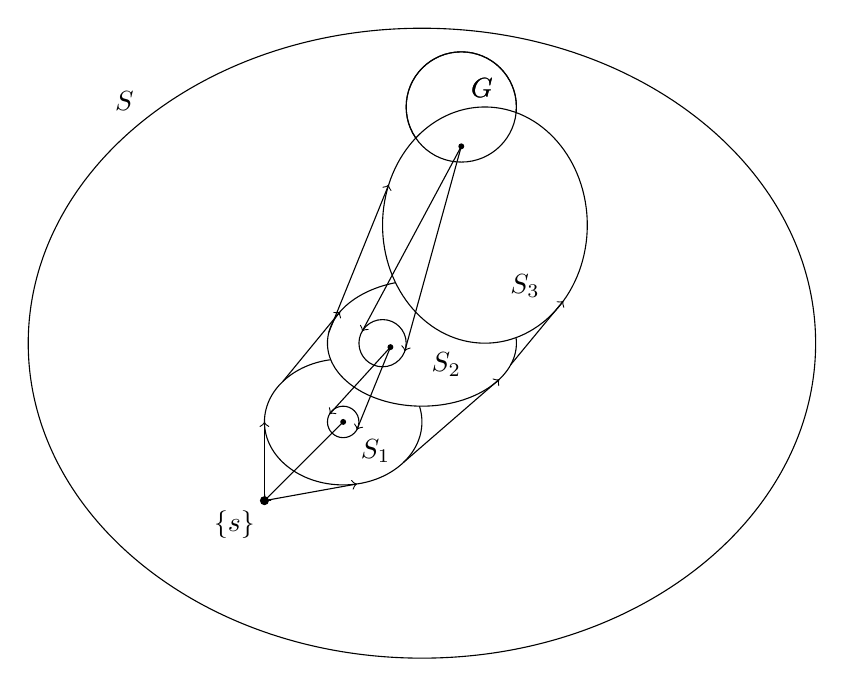
\begin{tikzpicture}

\draw (2,2) ellipse (5 and 4);
\node[above left] (S) at ($(2,2) + (135:5 and 4)$) {$S$};
\draw (2.5,5) node[above right]  {$G$} circle (.7);
\draw[fill] (0,0) node[below left] (S) {$\{s\}$} circle (.05); 
\pause
\draw[fill,color=white,draw=black] (1,1)  ellipse (1 and .8); 
\node[below right] (S1) at(1.1,.9) {$S_1$};
\draw[->] (0,0) -- ($(1,1) + (180:1 and .8)$);
\draw[->] (0,0) -- ($(1,1) + (-80:1 and .8)$);
\pause
\draw[fill,color=white,draw=black] (2,2) ellipse (1.2 and .8); 
\node[below right] (S2) at (2,2) {$S_2$};
\draw[->] ($(1,1) + (140:1 and .8)$) -- ($(2,2) + (150:1.2 and .8)$);
\draw[->] ($(1,1) + (-40:1 and .8)$) -- ($(2,2) + (-35:1.2 and .8)$);
\pause
\draw[fill,color=white,draw=black] (2.8,3.5)  ellipse (1.3 and 1.5); 
\node[below right] (S3) at (3,3) {$S_3$};
\draw[->] ($(2,2) + (170:1.2 and .8)$) -- ($(2.8,3.5) + (160:1.3 and 1.5)$);
\draw[->] ($(2,2) + (-20:1.2 and .8)$) -- ($(2.8,3.5) + (-40:1.3 and 1.5)$);

\draw (2.5,5) node[above right]  {$G$} circle (.7);

\pause
\draw[fill] (2.5,4.5) circle (.03); 
\pause
\draw (1.5,2) circle (.3); 
\draw[->] (2.5,4.5) -- ($(1.5,2) + (150:.3)$);
\draw[->] (2.5,4.5) -- ($(1.5,2) + (-20:.3)$);
\pause
\draw[fill] (1.6,1.95) circle (.03); 
\pause
\draw (1,1) circle (.2);
\draw[->] (1.6,1.95) -- ($(1,1) + (150:.2)$);
\draw[->] (1.6,1.95) -- ($(1,1) + (-30:.2)$);
\pause
\draw[fill] (1,1) circle (.03);
\draw[->] (1,1) -- (0,0);
\end{tikzpicture}

\end{frame}

\section{Adaptation of classical algorithms}
%\begin{frame}
%\frametitle{Symbolic shortest path search (Dijkstra)}
%
%We need to introduce Open(f,x) = true iff x is in the open list and has heuristic value f.
%
%  	  \begin{algorithmic}
%
%		%{\color<5-6>{gray}\color<handout>{black}
%			\STATE{$\t{Open}(f,x) \leftarrow (f=0) \land \Phi_{\{\t{init}\}}(x)$}
%			
%				\LOOP
%				
%        \STATE{$f_\t{min} \leftarrow \min \{ f | \exists f' \cdot f = f' \land
%                Open(f',x) \neq \t{false}(x)\} $}
%        \STATE{$\t{Min}(x) \leftarrow \exists f(\t{Open}(f,x) \land 
%                                              \lnot \t{Min}(x)$}
%                                              
%        \IF{$\t{Min}(x) \land\ \Phi_\t{Goal}(x) \neq \t{false}$}
%				  \RETURN{$\t{Build}(\t{Min}(x) \land \Phi_\t{Goal}(x))$}
%				\ENDIF				
%        
%				\STATE{$\t{Rest}(x) \leftarrow \t{Open}(f,x) \land \lnot\t{Min}(x)$}
%				\STATE{$\t{Succ}(f,x)$ $\leftarrow 
%				       \exists x,f',w \cdot$ 
%				       $\phantom{} \hspace{2.2cm} ( \t{Min}(x) \land Trans(w,x,x') \land
%				       f' = f_\t{min})[x \leftrightarrow x']$}
%				\STATE{$\t{Open}(x) \leftarrow \t{Rest}(f,x) \lor \t{Succ}(f,x) $}
%									
%				\ENDLOOP
%		%}
%		\end{algorithmic}
%\end{frame}
%
%\begin{frame}
%  	  \begin{algorithmic}
%
%		%{\color<5-6>{gray}\color<handout>{black}
%			\STATE{$\t{Open}(f,x) \leftarrow (f=0) \land \Phi_{\{\t{init}\}}(x)$}
%			
%				\LOOP
%				
%        \STATE{$f_\t{min} \leftarrow \min \{ f | \exists f' \cdot f = f' \land
%                Open(f',x) \neq \t{false}(x)\} $}
%        \STATE{$\t{Min}(x) \leftarrow \exists f(\t{Open}(f,x) \land 
%                                              \lnot \t{Min}(x)$}
%                                              
%        \IF{$\t{Min}(x) \land\ \Phi_\t{Goal}(x) \neq \t{false}$}
%				  \RETURN{$\t{Build}(\t{Min}(x) \land \Phi_\t{Goal}(x))$}
%				\ENDIF				
%        
%				\STATE{$\t{Rest}(x) \leftarrow \t{Open}(f,x) \land \lnot\t{Min}(x)$}
%				\STATE{$\t{Succ}(f,x)$ $\leftarrow 
%				       \exists w,x,h,h',f' \cdot ( \t{Min}(x) \land Trans(w,x,x') \land
%				       \t{Heur}(h,x) \land \t{Heur}(h',x') \land f'=f+w-h+h'
%				       \land f' = f_\t{min})[x \leftrightarrow x']$}
%				\STATE{$\t{Open}(x) \leftarrow \t{Rest}(f,x) \lor \t{Succ}(f,x) $}
%									
%				\ENDLOOP
%		%}
%		\end{algorithmic}
%
%\end{frame}

\begin{frame}
\frametitle{Dijkstra and A*}

Both use:
\begin{itemize}
\item a weighted transition relation: $\t{Trans}(w,x,x')$
\item a search frontier with heuristic values: $\t{Open}(f,x)$
\item a set of open nodes with minimal heuristic value: $\t{Min}(x)$ 
\end{itemize}

Difference between them: the successor computation.\\[.8cm]

Shortest Path (Dijkstra) -- $O(f^*)$\\[0.2cm]
$\t{Succ}(f,x)$ $\leftarrow 
			       \exists x,w \cdot$ 
				       $\phantom{} \hspace{1.2cm} ( \t{Min}(x) \land Trans(w,x,x') \land
				       f=f_\t{min}+w)[x \leftrightarrow x']$				       
				       \\[.8cm]
A* -- $O((f^*)^2)$\\[0.2cm]
$\t{Succ}(f,x)$ $\leftarrow 
				       \exists x,w,h,h' \cdot$\\
				       $\phantom{} \hspace{1.2cm} ( \t{Min}(x) \land Trans(w,x,x')$
				       $\phantom{} \hspace{1.2cm}
				       \land \t{Heur}(h,x) \land \t{Heur}(h',x') \land f=f_\t{min}+w-h+h')
				       [x \leftrightarrow x']$

\end{frame}

%\section{Fast pattern database with BBDs}
%\begin{frame}
%\frametitle{Fast pattern database with BBDs}
%
%BDDs are an efficient way to implement pattern databases.
%\begin{itemize}
%\item What is a pattern database ?
%\item How to implement it with BDDs ?
%\item Is it really so efficient ?
%\end{itemize}
%\end{frame}

\section{Conclusion}
\begin{frame}
\frametitle{Conclusion: BDDs and symbolic search}
\begin{itemize}
\item Compressed representation by sharing parts of the state vectors
\item Expected polynomial size to store exponential number of paths
\item Unique representation
\item Functionnal exploration: no need to uncompress the state sets
\end{itemize}
\end{frame}

\end{document}
